\documentclass[12pt, 3p]{elsarticle}
\usepackage{multirow}
\usepackage{array}
\usepackage{tikz}
\usepackage{pgfplots}
\usepackage{subfig}
\usepackage{threeparttable}
\usepackage{glossaries}
\usepackage{pdflscape}
\usepackage{listings}
\usepackage{url}

\usepackage[margin=10pt]{caption}


\usepackage{xcolor}

\lstset{
    language=Python,
    basicstyle=\ttfamily\small,             % Tamaño de fuente más pequeño para código
    keywordstyle=\color{blue}\bfseries,     % Palabras clave en azul y negrita
    commentstyle=\color{green},             % Comentarios en verde
    stringstyle=\color{red},                % Cadenas de texto en rojo
    backgroundcolor=\color{lightgray!20},   % Fondo gris claro para el código
    frame=single,                           % Marco alrededor del código
    rulecolor=\color{black!50},             % Color del marco
    numbers=left,                           % Números de línea a la izquierda
    numberstyle=\tiny\color{gray},          % Estilo de números de línea
    stepnumber=1,                           % Número de líneas incrementando de 1 en 1
    numbersep=5pt,                          % Separación entre los números y el código
    breaklines=true,                        % Rompe las líneas largas
    captionpos=b,                           % Título del código en la parte inferior
    showstringspaces=false,                 % No marcar los espacios en las cadenas
    aboveskip=10pt,                         % Espacio antes del código
    belowskip=10pt                          % Espacio después del código
}

\usetikzlibrary{arrows.meta}
\usetikzlibrary{datavisualization.formats.functions}
\pgfplotsset{compat=1.18}


\begin{document}

\title{Voltage Magnitude Impact of Residential Electric Vehicle Charging: 
A Case Study in Cusco, Peru}

\author[1]{Derian Carlos Tairo Garcia}
    \ead{d255905@dac.unicamp.br}
\author[1]{Erick Alberto Somocurcio Holguin} 
    \ead{e290883@dac.unicamp.br}

\affiliation[1]{organization=
    {Department of Systems and Energy (DSE), 
    School of Electrical and Computer Engineering (FEEC), 
    State University of Campinas (UNICAMP)},
    city={Campinas},
    state={São Paulo},
    country={Brazil}}
% \begin{abstract}
%     This is the abstract.
% \end{abstract}

% \begin{keyword}
%     electric vehicle charging \sep voltage magnitude \sep 
%     distribution grid 
% \end{keyword}

\begin{frontmatter}
    
\end{frontmatter}

\section{Introduction}\label{sec:introduction}

Cusco, the historical capital of the Inca Empire, stands today as 
one of South America's most prominent tourist destinations. With a 
population of approximately 430,000, the city experiences significant 
fluctuations in electricity demand, especially during the peak tourist 
season. These growing energy needs place substantial pressure 
on Cusco’s electrical infrastructure and energy supply systems.

Globally, the adoption of electric vehicles (EVs) has introduced 
various technical challenges, particularly in their integration into 
electrical distribution networks. The charging of EVs often affects 
the infrastructure, causing stress on local grids. However, in cities 
like Cusco, the secondary impacts of EV adoption remain largely 
unexplored. This study seeks to address this gap by offering a 
preliminary analysis of these effects on Cusco’s electrical grid.

One of the critical challenges faced during the study was the 
lack of a robust database necessary for performing computational 
simulations with tools like OpenDSS \cite{opendss}. 
Moreover, the absence of detailed 
demand profiles, inconsistencies in the database provided by the 
distribution system operator, and limited information on network 
topology posed additional hurdles. Georeferencing data was utilized 
to number the nodes, allowing for a partial reconstruction of the 
network model. To address these issues, several key actions were 
undertaken.

First, a database compatible with OpenDSS was developed to enable 
the simulation of EV connections to Cusco’s electrical distribution 
network. Various EV charging scenarios were then created and analyzed, 
including both public charging stations and private residential setups. 
These simulations were instrumental in assessing the impacts of EV 
integration on the network’s voltage profile. Additionally, corrective 
measures were modeled to address voltage violations observed during 
the simulations.

This study focuses on three primary objectives:

\begin{itemize}
    \item Develop a comprehensive database for OpenDSS simulations of EV integration.
    \item Simulate multiple EV charging scenarios to evaluate their grid impact.
    \item Analyze the technical effects, specifically voltage magnitude changes, resulting from EV adoption in Cusco’s electrical network.
\end{itemize}

The remainder of this paper is structured as follows:  
Section \ref{sec:methodology} describes the network model, 
EV and load profiles, and the creation of the circuit in OpenDSS.  
Section \ref{sec:cases} details the case studies used for analysis, 
with results presented in Section \ref{sec:results}.  
Finally, Section \ref{sec:conclusions} summarizes the 
main contributions of this study.
%  and outlines future research directions.

\section{Methodology}\label{sec:methodology}

This section begins by describing the distribution network
model used in this work. It then presents the EV and load
profiles, and lastly the creating of the circuit in OpenDSS.

\subsection{Network model}

Cusco is supplied by two main substations, Dolorespata and 
Quencoro, which together supplied the city's total demand. The 
substation under study is Quencoro (138/34.5/10.5 kV), 
located in the southern 
part of the city. Quencoro has seven feeders on the 10.5 kV 
side and three feeders on the 34.5 kV side, 
as shown in \ref{appndx:unifilar}.

For this analysis, the second feeder (QU-02) on the 10.5 kV 
side was selected. This feeder supplies power to 20 distribution 
transformers rated at 10.5/0.22 kV. Among these, the distribution 
transformer SED022 was chosen, which feeds three three-phase 
circuits and one public lighting circuit. The analysis focused 
on three-phase Circuit-03, which serves 117 single-phase customers 
distributed across phases (RS, ST, and TR). Load profiles were 
adapted for all customers at each load node to ensure accuracy.

The SED022 characteristics are shown in Table \ref{tab:system}
and the network model is shown in Fig. \ref{fig:network}.

\begin{table}[ht]
    \centering
    \caption{System Characteristics}
    \label{tab:system}
    \resizebox{\textwidth}{!}{
    \begin{tabular}{cccc}
    \hline
    \textbf{Customers (1-ph)} 
    & \textbf{LV Lines/Segments (3-ph)} 
    & \textbf{Distribution Transformer (3-ph)} 
    & \textbf{Frequency} \\ \hline
    117 & 24 & 10.5/0.22 kV/kV, 250 kVA (D-Y) & 60 Hz \\ 
    \hline
    \end{tabular}
    }
\end{table}

\begin{figure}[!ht]
    \centering
    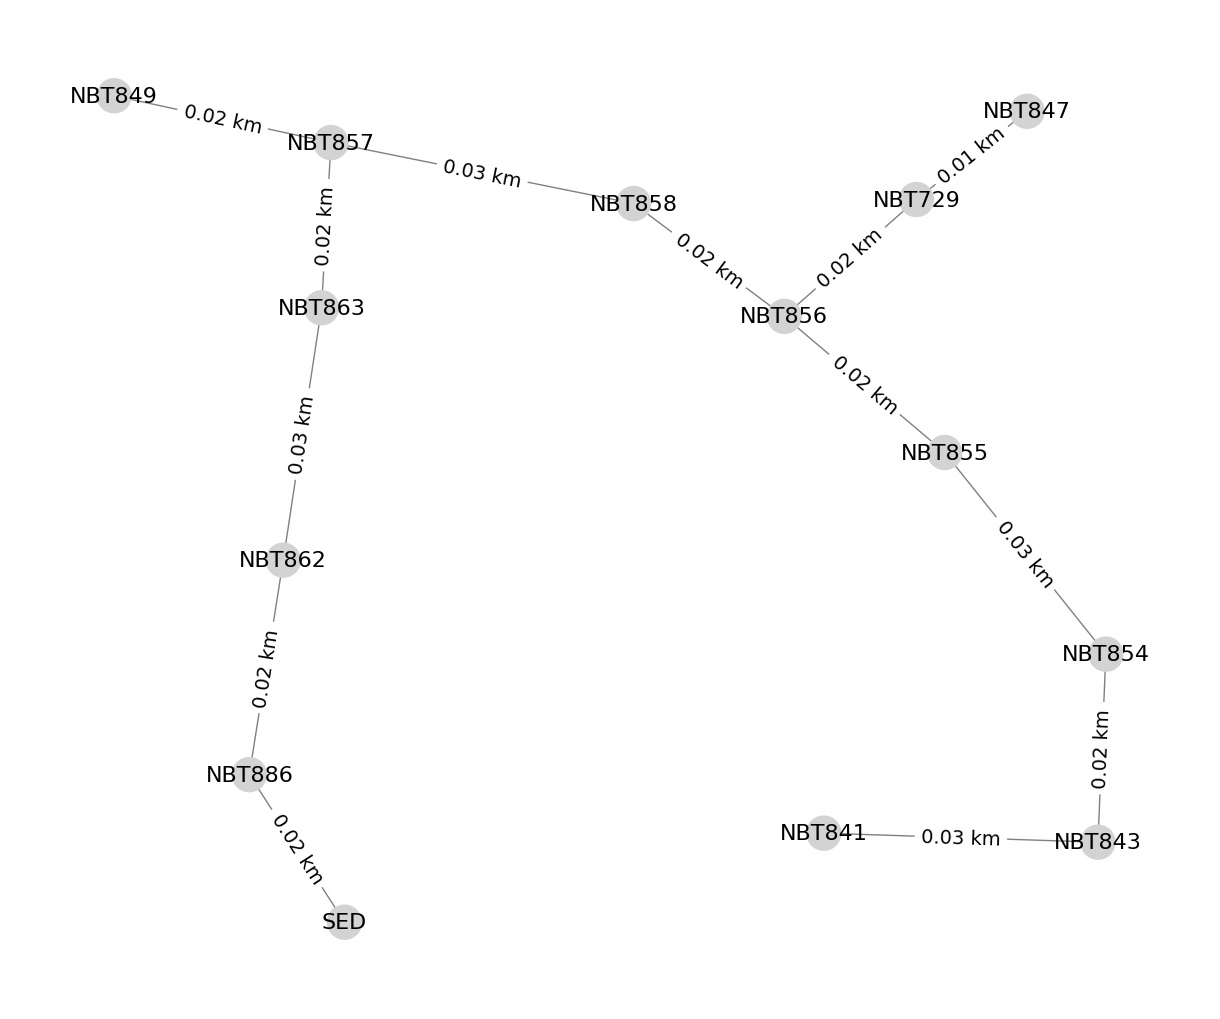
\includegraphics[width=0.8\textwidth]{./Figures/network.png}
    \caption{Substation SED022 grid model}
    \label{fig:network}
\end{figure}

To model the topology of the SED022 distribution network, 
a detailed and organized database was developed using data 
provided by the distribution system operator in Cusco 
(Electro Sur Este S.A.A.) \cite{ElectroSurEste}. The initial step 
involved exporting data into tables from ArcGIS \cite{ArcGIS10.3}, 
which included information on substations, nodes, lines, and 
customers. 

Next, the network topology was constructed using the geographic 
coordinates (latitude and longitude) of each node. The Python 
library \texttt{networkx} \cite{NetworkX} was employed to 
calculate the network's structure and the distances between 
nodes, as detailed in \ref{appndx:topology}.

This database served as the 
foundation for the network simulations and subsequent analyses.
    
\subsection{EV and load profiles}

The EV profiles were adapted from 
\cite{Richardson2013}. 
Figure \ref{fig:ev_profiles} illustrates three 
EV charging profiles: residential, 
workplace, and afternoon charging. These profiles were 
adjusted to reflect the characteristics of the BYD EV 
Dolphin \cite{byd}, as summarized in Table \ref{tab:byd_ev}. 
Finally, the profiles were scaled to align with the 
power ratings of the EVs in the dataset.

\begin{table}[!t]
    \centering
    \caption{Characteristics of the BYD EV Dolphin.}
    \label{tab:byd_ev}
    \begin{tabular}{lc}
        \hline
        \textbf{Feature} & \textbf{Specification} \\ \hline
        Battery capacity & 44.9 kWh \\ \hline
        AC charging power & 6.6 kW \\ \hline
        DC charging power & 60 kW \\ \hline
    \end{tabular}
\end{table}

Note that the charging time for each EV is approximately 7 
hours. Additionally, the afternoon charging profile is the 
only one specifically adapted for a 7-hour charging duration. 
The residential and workplace charging profiles extend to 10 
hours, as they align with typical residential and workplace 
schedules.

On the other hand, the load profiles were obtained 
from \cite{dataset_profiles}. Fig. \ref{fig:load_profiles} shows the 
load profiles adjusted for each of the 13 buses. Each profile is 
associated with a load node in the SED022 substation circuit. 
For this, the 117 customers were grouped into 13 load nodes, with 
each node representing an average load of 9 customers. This grouping 
ensures that the total load corresponds to the 117 customers.

\begin{figure}[!t]
    \centering
    \begin{tikzpicture}[baseline]
        \begin{axis}[
        xlabel={Period time [h]},
        ylabel near ticks,
        xlabel near ticks,
        ylabel={Active Power [p.u.]},
        % tick style = {line width = 0.5, color = lightgray, 
        %     major tick length=4pt,minor tick length=2pt,
        %     minor x tick num = 3, minor y tick num =1},
        % tick label style = {font=\small, xtick distance=1}
            % xticklabels={00:00, 00:00, 04:00, 08:00, 12:00, 16:00, 20:00},
        % label style = {},
        legend style = {font=\footnotesize, at={(0.99,0.98)}, 
            legend cell align=left, line width=0.5pt, draw=lightgray},
        % % legend entries={High PV, Medium PV, Low PV, High load, Medium load, Low load},
        % ymin=115, ymax=135,
        xmin=1, xmax=24,
        width=12cm,
        height=7.5cm,
        axis line style = {lightgray, line width = 0.5pt},
        cycle multi list={
        black\nextlist
        linestyles
        }
        ]
        \addplot  table 
            [col sep=comma, y=P1] {./Data/profiles_ev.dat};
        \addlegendentry[]{P1}
        \addplot  table 
            [col sep=comma, y=P2] {./Data/profiles_ev.dat};
        \addlegendentry[]{P2}
        \addplot  table 
            [col sep=comma, y=P3] {./Data/profiles_ev.dat};
        \addlegendentry[]{P3}

        \end{axis}
    \end{tikzpicture} 
    \caption{EV profiles}
    \label{fig:ev_profiles}
\end{figure}

\begin{figure}[!t]
    \centering
    \begin{tikzpicture}[baseline]
        \begin{axis}[
        xlabel={Period time [h]},
        ylabel near ticks,
        xlabel near ticks,
        ylabel={Voltage [p.u.]},
        % tick style = {line width = 0.5, color = lightgray, 
        %     major tick length=4pt,minor tick length=2pt,
        %     minor x tick num = 3, minor y tick num =1},
        % tick label style = {font=\small, xtick distance=4, 
        %     xticklabels={00:00, 00:00, 04:00, 08:00, 12:00, 16:00, 20:00}},
        % label style = {},
        legend style = {font=\footnotesize, at={(0.99,0.98)}, 
            legend cell align=left, line width=0.5pt, draw=lightgray, legend columns = 7},
        % ymin=115, ymax=135,
        xmin=1, xmax=24,
        width=12cm,
        height=7.5cm,
        axis line style = {lightgray, line width = 0.5pt},
        cycle multi list={
        lightgray, gray, black\nextlist
        linestyles
        }
        ]
        \addplot  table 
            [col sep=comma, y=P1] {./Data/profiles_load.dat};
        \addlegendentry[]{P1}
        \addplot  table 
            [col sep=comma, y=P2] {./Data/profiles_load.dat};
        \addlegendentry[]{P2}
        \addplot  table 
            [col sep=comma, y=P3] {./Data/profiles_load.dat};
        \addlegendentry[]{P3}
        \addplot  table 
            [col sep=comma, y=P4] {./Data/profiles_load.dat};
        \addlegendentry[]{P4}
        \addplot  table 
            [col sep=comma, y=P5] {./Data/profiles_load.dat};
        \addlegendentry[]{P5}
        \addplot  table 
            [col sep=comma, y=P6] {./Data/profiles_load.dat};
        \addlegendentry[]{P6}
        \addplot  table 
            [col sep=comma, y=P7] {./Data/profiles_load.dat};
        \addlegendentry[]{P7}
        \addplot  table 
            [col sep=comma, y=P8] {./Data/profiles_load.dat};
        \addlegendentry[]{P8}
        \addplot  table 
            [col sep=comma, y=P9] {./Data/profiles_load.dat};
        \addlegendentry[]{P9}
        \addplot  table 
            [col sep=comma, y=P10] {./Data/profiles_load.dat};
        \addlegendentry[]{P10}
        \addplot  table 
            [col sep=comma, y=P11] {./Data/profiles_load.dat};
        \addlegendentry[]{10}
        \addplot  table 
            [col sep=comma, y=P12] {./Data/profiles_load.dat};
        \addlegendentry[]{P12}
        \addplot  table 
            [col sep=comma, y=P13] {./Data/profiles_load.dat};
        \addlegendentry[]{P13}
        \end{axis}
    \end{tikzpicture} 
    \caption{Load profiles}
    \label{fig:load_profiles}
\end{figure}

\subsection{OpenDSS circuit creation}

The circuit was created in OpenDSS \cite{opendss} using the network 
model for the EV and load profiles, as explained in 
previous subsections. 

The Python library extension \texttt{dss} \cite{opendss_python} was 
used to automate the circuit creation process. Below is a summary of 
the code used to run the simulation. The complete implementation can 
be found in the repository referenced in Appendix \ref{appndx:repository}.

\begin{lstlisting}[caption={Python code to interact with OpenDSS}]
    import dss

    dss_engine = dss.DSS
    DSSText = dss_engine.Text                                                      
    DSSCircuit = dss_engine.ActiveCircuit                                            
    DSSSolution = dss_engine.ActiveCircuit.Solution                                  
    ControlQueue = dss_engine.ActiveCircuit.CtrlQueue                                           
    dss_engine.AllowForms = 0
    
    DSSText.Command = 'Clear'                             
    DSSText.Command = 'Compile ' + mydir +  '/Master.txt'    
    DSSText.Command = 'Set VoltageBases = [10.5, 0.22]'
    DSSText.Command = 'set controlmode=static'
    DSSText.Command = 'set mode=daily' 
    DSSText.Command = 'calcvoltagebases'
    
    DSSSolution.Solve()
    if DSSSolution.Converged:
        print("The Circuit was Successfully Solved")
\end{lstlisting}

\section{Cases studies}\label{sec:cases}

Two case studies were conducted to analyze the impact of
residential EV charging on the voltage magnitude of the
SED022 substation. The cases are as follows:

\begin{itemize}
    \item Case 1: Base case scenario with no EVs connected to the grid.
    \item Case 2: Scenario with 3 EVs (slow charging) connected to the grid.
\end{itemize}

It is important to mention that DC fast charging was not studied 
due to the focus on residential charging. Additionally, charging 
at public electric vehicle stations was not analyzed in this study.


\section{Results}\label{sec:results}
  
To analyze the results, the network under study was simulated 
to reflect its behavior as realistically as possible. The voltage 
magnitude was evaluated at the SED022 transformer output and at 
he NBT857, NBT856, and NBT841 buses to assess voltage drops 
throughout the network.

\begin{figure}
    \centering
    \begin{tikzpicture}[baseline]
        \begin{axis}[
        xlabel={Period time [h]},
        ylabel near ticks,
        xlabel near ticks,
        ylabel={Active Power [kW]},
        % tick style = {line width = 0.5, color = lightgray, 
        %     major tick length=4pt,minor tick length=2pt,
        %     minor x tick num = 3, minor y tick num =1},
        % tick label style = {font=\small, xtick distance=4, 
        %     xticklabels={00:00, 00:00, 04:00, 08:00, 12:00, 16:00, 20:00}},
        % label style = {},
        legend style = {font=\footnotesize, at={(0.99,0.98)}, 
            legend cell align=left, line width=0.5pt, draw=lightgray},
        % % legend entries={High PV, Medium PV, Low PV, High load, Medium load, Low load},
        % ymin=115, ymax=135,
        xmin=1, xmax=24,
        width=12cm,
        height=7.5cm,
        axis line style = {lightgray, line width = 0.5pt},
        cycle multi list={
        black\nextlist
        linestyles
        }
        ]
        \addplot  table 
            [col sep=comma, y=P1] {./Data/SED_base.dat};
        \addlegendentry[]{$P_{123}^{Base}$}
        \addplot  table 
            [col sep=comma, y=P2] {./Data/SED_base.dat};
        \addlegendentry[]{$P_{123}^{EVs}$}
        \addplot  table 
            [col sep=comma, y=P3] {./Data/SED_base.dat};
        \addlegendentry[]{$P_{123}^{Corrective}$}
    
        \end{axis}
    \end{tikzpicture} 
    \caption{Load profile at the SED022 transformer for Case I, II and corrective solution.}
    \label{fig:case_I_peak}
\end{figure}

In Case I, the voltage profile shows minimal variations at 
the substation output. However, midway through the network 
(see Fig.~\ref{fig:case_I_NBT857}), voltage variations start 
to appear. At the last node, NBT841 (Fig.~\ref{fig:case_I_NBT841}), 
a more significant voltage drop is observed. This is primarily due 
to the peak demand period, as shown in Fig.~\ref{fig:case_I_peak}. 
During other periods, these voltage variations are less pronounced. 
Figure~\ref{fig:case_I_base} presents the overall voltage 
magnitudes for the studied nodes and the SED022 transformer.

In Case II, three EVs were added to the studied nodes 
(NBT857, NBT856, and NBT841). It is important to note 
that the demand profile, with the inclusion of EVs and 
their varying charging schedules, accentuates these 
voltage drops. Additionally, the last nodes experience a 
more significant voltage magnitude impact, as well as 
voltage imbalance between phases, as shown in 
Fig.~\ref{fig:case_II_base}.


\begin{figure}[!ht]
    \centering
    \resizebox{\textwidth}{!}{%
        \begin{tabular}{cc}
            \subfloat[Case I: Voltage magnitudes at the SED022 transformer output.]{
                \begin{tikzpicture}[baseline]
    \begin{axis}[
    xlabel={Period time [h]},
    ylabel near ticks,
    xlabel near ticks,
    ylabel={Voltage [V]},
    % tick style = {line width = 0.5, color = lightgray, 
    %     major tick length=4pt,minor tick length=2pt,
    %     minor x tick num = 3, minor y tick num =1},
    % tick label style = {font=\small, xtick distance=4, 
    %     xticklabels={00:00, 00:00, 04:00, 08:00, 12:00, 16:00, 20:00}},
    % label style = {},
    legend style = {font=\footnotesize, at={(0.99,0.98)}, 
        legend cell align=left, line width=0.5pt, draw=lightgray, 
        legend columns=3},
    ymin=120, ymax=134.5,
    xmin=01, xmax=24,
    width=12cm,
    height=7.5cm,
    axis line style = {lightgray, line width = 0.5pt},
    cycle multi list={
    black\nextlist
    linestyles
    }
    ]
    \addplot  table 
        [col sep=comma, y=V1] {./Data/SED_base.dat};
    \addlegendentry[]{$V_{1}$}
    \addplot  table 
        [col sep=comma, y=V2] {./Data/SED_base.dat};
    \addlegendentry[]{$V_{2}$}
    \addplot  table 
        [col sep=comma, y=V3] {./Data/SED_base.dat};
    \addlegendentry[]{$V_{3}$}

    \addplot  table 
        [col sep=comma, y=Vmin] {./Data/SED_base.dat}; 
    \addlegendentry{$V_{min}$}     
    \addplot  table 
        [col sep=comma, y=Vmax] {./Data/SED_base.dat}; 
    \addlegendentry{$V_{max}$}     

    \end{axis}
\end{tikzpicture} 
                \label{fig:case_I_SED}
            } &
            \subfloat[Case I: Voltage magnitudes at the NBT857 bus.]{
                \begin{tikzpicture}[baseline]
    \begin{axis}[
    xlabel={Period time [h]},
    ylabel near ticks,
    xlabel near ticks,
    ylabel={Voltage [V]},
    % tick style = {line width = 0.5, color = lightgray, 
    %     major tick length=4pt,minor tick length=2pt,
    %     minor x tick num = 3, minor y tick num =1},
    % tick label style = {font=\small, xtick distance=4, 
    %     xticklabels={00:00, 00:00, 04:00, 08:00, 12:00, 16:00, 20:00}},
    % label style = {},
    legend style = {font=\footnotesize, at={(0.99,0.98)}, 
        legend cell align=left, line width=0.5pt, draw=lightgray, 
        legend columns=3},
    ymin=120, ymax=134.5,
    xmin=01, xmax=24,
    width=12cm,
    height=7.5cm,
    axis line style = {lightgray, line width = 0.5pt},
    cycle multi list={
    black\nextlist
    linestyles
    }
    ]
    \addplot  table 
        [col sep=comma, y=V1] {./Data/NBT857_base.dat};
    \addlegendentry[]{$V_{1}$}
    \addplot  table 
        [col sep=comma, y=V2] {./Data/NBT857_base.dat};
    \addlegendentry[]{$V_{2}$}
    \addplot  table 
        [col sep=comma, y=V3] {./Data/NBT857_base.dat};
    \addlegendentry[]{$V_{3}$}

    \addplot [gray, mark = triangle] table 
        [col sep=comma, y=Vmin] {./Data/NBT857_base.dat}; 
    \addlegendentry{$V_{min}$}     
    \addplot [gray, mark = square] table 
        [col sep=comma, y=Vmax] {./Data/NBT857_base.dat}; 
    \addlegendentry{$V_{max}$}        

    \end{axis}
\end{tikzpicture} 
                \label{fig:case_I_NBT857}
            } \\
            \subfloat[Case I: Voltage magnitudes at the NBT856 bus.]{
                \begin{tikzpicture}[baseline]
    \begin{axis}[
    xlabel={Period time [h]},
    ylabel near ticks,
    xlabel near ticks,
    ylabel={Voltage [V]},
    % tick style = {line width = 0.5, color = lightgray, 
    %     major tick length=4pt,minor tick length=2pt,
    %     minor x tick num = 3, minor y tick num =1},
    % tick label style = {font=\small, xtick distance=4, 
    %     xticklabels={00:00, 00:00, 04:00, 08:00, 12:00, 16:00, 20:00}},
    % label style = {},
    legend style = {font=\footnotesize, at={(0.99,0.98)}, 
        legend cell align=left, line width=0.5pt, draw=lightgray, 
        legend columns=3},
    ymin=120, ymax=134.5,
    xmin=01, xmax=24,
    width=12cm,
    height=7.5cm,
    axis line style = {lightgray, line width = 0.5pt},
    cycle multi list={
    black\nextlist
    linestyles
    }
    ]
    \addplot  table 
        [col sep=comma, y=V1] {./Data/NBT856_base.dat};
    \addlegendentry[]{$V_{1}$}
    \addplot  table 
        [col sep=comma, y=V2] {./Data/NBT856_base.dat};
    \addlegendentry[]{$V_{2}$}
    \addplot  table 
        [col sep=comma, y=V3] {./Data/NBT856_base.dat};
    \addlegendentry[]{$V_{3}$}

    \addplot [gray, mark = triangle] table 
        [col sep=comma, y=Vmin] {./Data/NBT857_base.dat}; 
    \addlegendentry{$V_{min}$}     
    \addplot [gray, mark = square] table 
        [col sep=comma, y=Vmax] {./Data/NBT857_base.dat}; 
    \addlegendentry{$V_{max}$}       

    \end{axis}
\end{tikzpicture} 
                \label{fig:case_I_NBT856}
            } &
            \subfloat[Case I: Voltage magnitudes at the NBT841 bus.]{
                \begin{tikzpicture}[baseline]
    \begin{axis}[
    xlabel={Period time [h]},
    ylabel near ticks,
    xlabel near ticks,
    ylabel={Voltage [V]},
    % tick style = {line width = 0.5, color = lightgray, 
    %     major tick length=4pt,minor tick length=2pt,
    %     minor x tick num = 3, minor y tick num =1},
    % tick label style = {font=\small, xtick distance=4, 
    %     xticklabels={00:00, 00:00, 04:00, 08:00, 12:00, 16:00, 20:00}},
    % label style = {},
    legend style = {font=\footnotesize, at={(0.99,0.98)}, 
        legend cell align=left, line width=0.5pt, draw=lightgray, 
        legend columns=3},
    ymin=120, ymax=134.5,
    xmin=01, xmax=24,
    width=12cm,
    height=7.5cm,
    axis line style = {lightgray, line width = 0.5pt},
    cycle multi list={
    black\nextlist
    linestyles
    }
    ]
    \addplot  table 
        [col sep=comma, y=V1] {./Data/NBT841_base.dat};
    \addlegendentry[]{$V_{1}$}
    \addplot  table 
        [col sep=comma, y=V2] {./Data/NBT841_base.dat};
    \addlegendentry[]{$V_{2}$}
    \addplot  table 
        [col sep=comma, y=V3] {./Data/NBT841_base.dat};
    \addlegendentry[]{$V_{3}$}

    \addplot [gray, mark = triangle] table 
        [col sep=comma, y=Vmin] {./Data/NBT857_base.dat}; 
    \addlegendentry{$V_{min}$}     
    \addplot [gray, mark = square] table 
        [col sep=comma, y=Vmax] {./Data/NBT857_base.dat}; 
    \addlegendentry{$V_{max}$}      

    \end{axis}
\end{tikzpicture} 
                \label{fig:case_I_NBT841}
            }
        \end{tabular}
    }
    \caption{Case I: Voltage magnitudes.}
    \label{fig:case_I_base}
\end{figure}


The next subsection explained the corrective solutions.

\begin{figure}[!ht]
    \centering
    \resizebox{\textwidth}{!}{%
        \begin{tabular}{cc}
            \subfloat[Case II: Voltage magnitudes at the SED022 transformer output.]{
                \begin{tikzpicture}[baseline]
    \begin{axis}[
    xlabel={Period time [h]},
    ylabel near ticks,
    xlabel near ticks,
    ylabel={Voltage [V]},
    % tick style = {line width = 0.5, color = lightgray, 
    %     major tick length=4pt,minor tick length=2pt,
    %     minor x tick num = 3, minor y tick num =1},
    % tick label style = {font=\small, xtick distance=4, 
    %     xticklabels={00:00, 00:00, 04:00, 08:00, 12:00, 16:00, 20:00}},
    % label style = {},
    legend style = {font=\footnotesize, at={(0.99,0.98)}, 
        legend cell align=left, line width=0.5pt, draw=lightgray, 
        legend columns=3},
    ymin=120, ymax=134.5,
    xmin=01, xmax=24,
    width=12cm,
    height=7.5cm,
    axis line style = {lightgray, line width = 0.5pt},
    cycle multi list={
    lightgray, black\nextlist
    linestyles
    }
    ]
    \addplot  table 
        [col sep=comma, y=V1] {./Data/SED_base.dat};
    \addlegendentry[]{$V_{1}$}
    \addplot  table 
        [col sep=comma, y=V2] {./Data/SED_base.dat};
    \addlegendentry[]{$V_{2}$}
    \addplot  table 
        [col sep=comma, y=V3] {./Data/SED_base.dat};
    \addlegendentry[]{$V_{3}$}

    \addplot  table 
        [col sep=comma, y=V1ev] {./Data/SED_base.dat};
    \addlegendentry[]{$V_{1}^{EV}$}
    \addplot  table 
        [col sep=comma, y=V2ev] {./Data/SED_base.dat};
    \addlegendentry[]{$V_{2}^{EV}$}
    \addplot  table 
        [col sep=comma, y=V3ev] {./Data/SED_base.dat};
    \addlegendentry[]{$V_{3}^{EV}$}

    \addplot [gray, mark = triangle] table 
        [col sep=comma, y=Vmin] {./Data/NBT857_base.dat}; 
    \addlegendentry{$V_{min}$}     
    \addplot [gray, mark = square] table 
        [col sep=comma, y=Vmax] {./Data/NBT857_base.dat}; 
    \addlegendentry{$V_{max}$}  
    \end{axis}
\end{tikzpicture} 
                \label{fig:case_II_SED}
            } &
            \subfloat[Case II: Voltage magnitudes at the NBT857 bus.]{
                \begin{tikzpicture}[baseline]
    \begin{axis}[
    xlabel={Period time [h]},
    ylabel near ticks,
    xlabel near ticks,
    ylabel={Voltage [V]},
    % tick style = {line width = 0.5, color = lightgray, 
    %     major tick length=4pt,minor tick length=2pt,
    %     minor x tick num = 3, minor y tick num =1},
    % tick label style = {font=\small, xtick distance=4, 
    %     xticklabels={00:00, 00:00, 04:00, 08:00, 12:00, 16:00, 20:00}},
    % label style = {},
    legend style = {font=\footnotesize, at={(0.99,0.98)}, 
        legend cell align=left, line width=0.5pt, draw=lightgray, 
        legend columns=3},
    ymin=120, ymax=134.5,
    xmin=01, xmax=24,
    width=12cm,
    height=7.5cm,
    axis line style = {lightgray, line width = 0.5pt},
    cycle multi list={
    lightgray, black\nextlist
    linestyles
    }
    ]
    \addplot table 
        [col sep=comma, y=V1] {./Data/NBT857_base.dat};
    \addlegendentry[]{$V_{1}$}
    \addplot table 
        [col sep=comma, y=V2] {./Data/NBT857_base.dat};
    \addlegendentry[]{$V_{2}$}
    \addplot table 
        [col sep=comma, y=V3] {./Data/NBT857_base.dat};
    \addlegendentry[]{$V_{3}$}

    \addplot  table 
        [col sep=comma, y=V1ev] {./Data/NBT857_base.dat};
    \addlegendentry[]{$V_{1}^{EV}$}
    \addplot  table 
        [col sep=comma, y=V2ev] {./Data/NBT857_base.dat};
    \addlegendentry[]{$V_{2}^{EV}$}
    \addplot table 
        [col sep=comma, y=V3ev] {./Data/NBT857_base.dat};
    \addlegendentry[]{$V_{3}^{EV}$}

    \addplot [gray, mark = triangle] table 
        [col sep=comma, y=Vmin] {./Data/NBT857_base.dat}; 
    \addlegendentry{$V_{min}$}     
    \addplot [gray, mark = square] table 
        [col sep=comma, y=Vmax] {./Data/NBT857_base.dat}; 
    \addlegendentry{$V_{max}$}     

    \end{axis}
\end{tikzpicture} 
                \label{fig:case_II_NBT857}
            } \\
            \subfloat[Case II: Voltage magnitudes at the NBT856 bus.]{
                \begin{tikzpicture}[baseline]
    \begin{axis}[
    xlabel={Period time [h]},
    ylabel near ticks,
    xlabel near ticks,
    ylabel={Voltage [V]},
    % tick style = {line width = 0.5, color = lightgray, 
    %     major tick length=4pt,minor tick length=2pt,
    %     minor x tick num = 3, minor y tick num =1},
    % tick label style = {font=\small, xtick distance=4, 
    %     xticklabels={00:00, 00:00, 04:00, 08:00, 12:00, 16:00, 20:00}},
    % label style = {},
    legend style = {font=\footnotesize, at={(0.99,0.98)}, 
        legend cell align=left, line width=0.5pt, draw=lightgray, 
        legend columns=3},
    ymin=120, ymax=134.5,
    xmin=01, xmax=24,
    width=12cm,
    height=7.5cm,
    axis line style = {lightgray, line width = 0.5pt},
    cycle multi list={
    lightgray, black\nextlist
    linestyles
    }
    ]
    \addplot  table 
        [col sep=comma, y=V1] {./Data/NBT856_base.dat};
    \addlegendentry[]{$V_{1}$}
    \addplot  table 
        [col sep=comma, y=V2] {./Data/NBT856_base.dat};
    \addlegendentry[]{$V_{2}$}
    \addplot  table 
        [col sep=comma, y=V3] {./Data/NBT856_base.dat};
    \addlegendentry[]{$V_{3}$}

    \addplot  table 
        [col sep=comma, y=V1ev] {./Data/NBT856_base.dat};
    \addlegendentry[]{$V_{1}^{EV}$}
    \addplot  table 
        [col sep=comma, y=V2ev] {./Data/NBT856_base.dat};
    \addlegendentry[]{$V_{2}^{EV}$}
    \addplot  table 
        [col sep=comma, y=V3ev] {./Data/NBT856_base.dat};
    \addlegendentry[]{$V_{3}^{EV}$}

    \addplot [gray, mark = triangle] table 
        [col sep=comma, y=Vmin] {./Data/NBT857_base.dat}; 
    \addlegendentry{$V_{min}$}     
    \addplot [gray, mark = square] table 
        [col sep=comma, y=Vmax] {./Data/NBT857_base.dat}; 
    \addlegendentry{$V_{max}$}     

    \end{axis}
\end{tikzpicture} 
                \label{fig:case_II_NBT856}
            } &
            \subfloat[Case II: Voltage magnitudes at the NBT841 bus.]{
                \begin{tikzpicture}[baseline]
    \begin{axis}[
    xlabel={Period time [h]},
    ylabel near ticks,
    xlabel near ticks,
    ylabel={Voltage [V]},
    % tick style = {line width = 0.5, color = lightgray, 
    %     major tick length=4pt,minor tick length=2pt,
    %     minor x tick num = 3, minor y tick num =1},
    % tick label style = {font=\small, xtick distance=4, 
    %     xticklabels={00:00, 00:00, 04:00, 08:00, 12:00, 16:00, 20:00}},
    % label style = {},
    legend style = {font=\footnotesize, at={(0.99,0.98)}, 
        legend cell align=left, line width=0.5pt, draw=lightgray, 
        legend columns=3},
    ymin=120, ymax=134.5,
    xmin=01, xmax=24,
    width=12cm,
    height=7.5cm,
    axis line style = {lightgray, line width = 0.5pt},
    cycle multi list={
    lightgray, black\nextlist
    linestyles
    }
    ]
    \addplot  table 
        [col sep=comma, y=V1] {./Data/NBT841_base.dat};
    \addlegendentry[]{$V_{1}$}
    \addplot  table 
        [col sep=comma, y=V2] {./Data/NBT841_base.dat};
    \addlegendentry[]{$V_{2}$}
    \addplot  table 
        [col sep=comma, y=V3] {./Data/NBT841_base.dat};
    \addlegendentry[]{$V_{3}$}

    \addplot table 
        [col sep=comma, y=V1ev] {./Data/NBT841_base.dat};
    \addlegendentry[]{$V_{1}^{EV}$}
    \addplot  table 
        [col sep=comma, y=V2ev] {./Data/NBT841_base.dat};
    \addlegendentry[]{$V_{2}^{EV}$}
    \addplot  table 
        [col sep=comma, y=V3ev] {./Data/NBT841_base.dat};
    \addlegendentry[]{$V_{3}^{EV}$}

    \addplot [gray, mark = triangle] table 
        [col sep=comma, y=Vmin] {./Data/NBT857_base.dat}; 
    \addlegendentry{$V_{min}$}     
    \addplot [gray, mark = square] table 
        [col sep=comma, y=Vmax] {./Data/NBT857_base.dat}; 
    \addlegendentry{$V_{max}$}    

    \end{axis}
\end{tikzpicture} 
                \label{fig:case_II_NBT841}
            }
        \end{tabular}
    }
    \caption{Case II: Voltage magnitudes.}
    \label{fig:case_II_base}
\end{figure}

\subsection{Corrective solutions}

To mitigate the impacts of EV charging on 
the voltage profile, 
two corrective measures were analyzed. These solutions aimed 
to address voltage violations and ensure the magnitude of voltage 
acrros the entire grid.

The corrective measures implemented were:  

\begin{itemize}
    \item Converting the charging of the three EVs to a three-phase load. 
    \item Increasing the conductor's cross-sectional area 
    ($25 mm^{2}$ to $120 mm^{2}$). 
\end{itemize}
 
These actions successfully mitigated the voltage magnitude drop 
at the studied nodes, as shown in Fig.~\ref{fig:case_III_base}.

\begin{figure}[!ht]
    \centering
    \resizebox{\textwidth}{!}{%
        \begin{tabular}{cc}
            \subfloat[Voltage magnitudes at the SED022 transformer output.]{
                \begin{tikzpicture}[baseline]
    \begin{axis}[
    xlabel={Period time [h]},
    ylabel near ticks,
    xlabel near ticks,
    ylabel={Voltage [V]},
    % tick style = {line width = 0.5, color = lightgray, 
    %     major tick length=4pt,minor tick length=2pt,
    %     minor x tick num = 3, minor y tick num =1},
    % tick label style = {font=\small, xtick distance=4, 
    %     xticklabels={00:00, 00:00, 04:00, 08:00, 12:00, 16:00, 20:00}},
    % label style = {},
    legend style = {font=\footnotesize, at={(0.99,0.98)}, 
        legend cell align=left, line width=0.5pt, draw=lightgray, 
        legend columns=3},
    ymin=120, ymax=134.5,
    xmin=01, xmax=24,
    width=12cm,
    height=7.5cm,
    axis line style = {lightgray, line width = 0.5pt},
    cycle multi list={
    lightgray, black\nextlist
    linestyles
    }
    ]

    \addplot table 
        [col sep=comma, y=V1ev] {./Data/SED_base.dat};
    \addlegendentry[]{$V_{1}^{EV}$}
    \addplot table 
        [col sep=comma, y=V2ev] {./Data/SED_base.dat};
    \addlegendentry[]{$V_{2}^{EV}$}
    \addplot table 
        [col sep=comma, y=V3ev] {./Data/SED_base.dat};
    \addlegendentry[]{$V_{3}^{EV}$}

    \addplot table 
        [col sep=comma, y=V1c] {./Data/SED_base.dat};
    \addlegendentry[]{$V_{1}^{EV}$}
    \addplot table 
        [col sep=comma, y=V2c] {./Data/SED_base.dat};
    \addlegendentry[]{$V_{2}^{EV}$}
    \addplot table 
        [col sep=comma, y=V3c] {./Data/SED_base.dat};
    \addlegendentry[]{$V_{3}^{EV}$}

    \addplot [gray, mark = triangle] table 
        [col sep=comma, y=Vmin] {./Data/NBT857_base.dat}; 
    \addlegendentry{$V_{min}$}     
    \addplot [gray, mark = square] table 
        [col sep=comma, y=Vmax] {./Data/NBT857_base.dat}; 
    \addlegendentry{$V_{max}$}  
    \end{axis}
\end{tikzpicture} 
                \label{fig:case_III_SED}
            } &
            \subfloat[Voltage magnitudes at the NBT857 bus.]{
                \begin{tikzpicture}[baseline]
    \begin{axis}[
    xlabel={Period time [h]},
    ylabel near ticks,
    xlabel near ticks,
    ylabel={Voltage [V]},
    % tick style = {line width = 0.5, color = lightgray, 
    %     major tick length=4pt,minor tick length=2pt,
    %     minor x tick num = 3, minor y tick num =1},
    % tick label style = {font=\small, xtick distance=4, 
    %     xticklabels={00:00, 00:00, 04:00, 08:00, 12:00, 16:00, 20:00}},
    % label style = {},
    legend style = {font=\footnotesize, at={(0.99,0.98)}, 
        legend cell align=left, line width=0.5pt, draw=lightgray, 
        legend columns=3},
    ymin=120, ymax=134.5,
    xmin=01, xmax=24,
    width=12cm,
    height=7.5cm,
    axis line style = {lightgray, line width = 0.5pt},
    cycle multi list={
    lightgray, black\nextlist
    linestyles
    }
    ]

    \addplot  table 
        [col sep=comma, y=V1ev] {./Data/NBT857_base.dat};
    \addlegendentry[]{$V_{1}^{EV}$}
    \addplot  table 
        [col sep=comma, y=V2ev] {./Data/NBT857_base.dat};
    \addlegendentry[]{$V_{2}^{EV}$}
    \addplot table 
        [col sep=comma, y=V3ev] {./Data/NBT857_base.dat};
    \addlegendentry[]{$V_{3}^{EV}$}

    \addplot  table 
        [col sep=comma, y=V1c] {./Data/NBT857_base.dat};
    \addlegendentry[]{$V_{1}^{EV}$}
    \addplot  table 
        [col sep=comma, y=V2c] {./Data/NBT857_base.dat};
    \addlegendentry[]{$V_{2}^{EV}$}
    \addplot table 
        [col sep=comma, y=V3c] {./Data/NBT857_base.dat};
    \addlegendentry[]{$V_{3}^{EV}$}

    \addplot [gray, mark = triangle] table 
        [col sep=comma, y=Vmin] {./Data/NBT857_base.dat}; 
    \addlegendentry{$V_{min}$}     
    \addplot [gray, mark = square] table 
        [col sep=comma, y=Vmax] {./Data/NBT857_base.dat}; 
    \addlegendentry{$V_{max}$}     

    \end{axis}
\end{tikzpicture} 
                \label{fig:case_III_NBT857}
            } \\
            \subfloat[Voltage magnitudes at the NBT856 bus.]{
                \begin{tikzpicture}[baseline]
    \begin{axis}[
    xlabel={Period time [h]},
    ylabel near ticks,
    xlabel near ticks,
    ylabel={Voltage [V]},
    % tick style = {line width = 0.5, color = lightgray, 
    %     major tick length=4pt,minor tick length=2pt,
    %     minor x tick num = 3, minor y tick num =1},
    % tick label style = {font=\small, xtick distance=4, 
    %     xticklabels={00:00, 00:00, 04:00, 08:00, 12:00, 16:00, 20:00}},
    % label style = {},
    legend style = {font=\footnotesize, at={(0.99,0.98)}, 
        legend cell align=left, line width=0.5pt, draw=lightgray, 
        legend columns=3},
    ymin=120, ymax=134.5,
    xmin=01, xmax=24,
    width=12cm,
    height=7.5cm,
    axis line style = {lightgray, line width = 0.5pt},
    cycle multi list={
    lightgray, black\nextlist
    linestyles
    }
    ]

    \addplot  table 
        [col sep=comma, y=V1ev] {./Data/NBT856_base.dat};
    \addlegendentry[]{$V_{1}^{EV}$}
    \addplot  table 
        [col sep=comma, y=V2ev] {./Data/NBT856_base.dat};
    \addlegendentry[]{$V_{2}^{EV}$}
    \addplot  table 
        [col sep=comma, y=V3ev] {./Data/NBT856_base.dat};
    \addlegendentry[]{$V_{3}^{EV}$}

    \addplot  table 
        [col sep=comma, y=V1c] {./Data/NBT856_base.dat};
    \addlegendentry[]{$V_{1}^{EV}$}
    \addplot  table 
        [col sep=comma, y=V2c] {./Data/NBT856_base.dat};
    \addlegendentry[]{$V_{2}^{EV}$}
    \addplot  table 
        [col sep=comma, y=V3c] {./Data/NBT856_base.dat};
    \addlegendentry[]{$V_{3}^{EV}$}

    \addplot [gray, mark = triangle] table 
        [col sep=comma, y=Vmin] {./Data/NBT857_base.dat}; 
    \addlegendentry{$V_{min}$}     
    \addplot [gray, mark = square] table 
        [col sep=comma, y=Vmax] {./Data/NBT857_base.dat}; 
    \addlegendentry{$V_{max}$}     

    \end{axis}
\end{tikzpicture} 
                \label{fig:case_III_NBT856}
            } &
            \subfloat[Voltage magnitudes at the NBT841 bus.]{
                \begin{tikzpicture}[baseline]
    \begin{axis}[
    xlabel={Period time [h]},
    ylabel near ticks,
    xlabel near ticks,
    ylabel={Voltage [V]},
    % tick style = {line width = 0.5, color = lightgray, 
    %     major tick length=4pt,minor tick length=2pt,
    %     minor x tick num = 3, minor y tick num =1},
    % tick label style = {font=\small, xtick distance=4, 
    %     xticklabels={00:00, 00:00, 04:00, 08:00, 12:00, 16:00, 20:00}},
    % label style = {},
    legend style = {font=\footnotesize, at={(0.99,0.98)}, 
        legend cell align=left, line width=0.5pt, draw=lightgray, 
        legend columns=3},
    ymin=120, ymax=134.5,
    xmin=01, xmax=24,
    width=12cm,
    height=7.5cm,
    axis line style = {lightgray, line width = 0.5pt},
    cycle multi list={
    lightgray, black\nextlist
    linestyles
    }
    ]

    \addplot table 
        [col sep=comma, y=V1ev] {./Data/NBT841_base.dat};
    \addlegendentry[]{$V_{1}^{EV}$}
    \addplot  table 
        [col sep=comma, y=V2ev] {./Data/NBT841_base.dat};
    \addlegendentry[]{$V_{2}^{EV}$}
    \addplot  table 
        [col sep=comma, y=V3ev] {./Data/NBT841_base.dat};
    \addlegendentry[]{$V_{3}^{EV}$}
    
    \addplot table 
        [col sep=comma, y=V1c] {./Data/NBT841_base.dat};
    \addlegendentry[]{$V_{1}^{EV}$}
    \addplot  table 
        [col sep=comma, y=V2c] {./Data/NBT841_base.dat};
    \addlegendentry[]{$V_{2}^{EV}$}
    \addplot  table 
        [col sep=comma, y=V3c] {./Data/NBT841_base.dat};
    \addlegendentry[]{$V_{3}^{EV}$}

    \addplot [gray, mark = triangle] table 
        [col sep=comma, y=Vmin] {./Data/NBT857_base.dat}; 
    \addlegendentry{$V_{min}$}     
    \addplot [gray, mark = square] table 
        [col sep=comma, y=Vmax] {./Data/NBT857_base.dat}; 
    \addlegendentry{$V_{max}$}    

    \end{axis}
\end{tikzpicture} 
                \label{fig:case_III_NBT841}
            }
        \end{tabular}
    }
    \caption{Corrective solution for voltage magnitudes.}
    \label{fig:case_III_base}
\end{figure}


\section{Conclusions}\label{sec:conclusions}
    

This work presented a preliminary analysis of the impact of 
electric vehicle (EV) charging on the electrical distribution 
network in Cusco. The results demonstrated that:

\begin{itemize}
    \item The integration of electric vehicles into the grid can significantly affect the voltage profile, particularly during peak demand periods. This effect is more pronounced at nodes farther from the substation, where voltage drops become more evident.
    \item Simulating various charging scenarios revealed that the addition of EVs leads to increased voltage variation, especially at the last nodes in the network. This issue is further exacerbated by the lack of adequate infrastructure to handle the increased demand.
    \item Corrective measures, such as converting to a three-phase load and increasing the conductor cross-section, were found to effectively mitigate the voltage drop, ensuring that voltage levels remain within acceptable limits.
    \item The study also highlighted the importance of incorporating realistic demand profiles and charging schedules for EVs to accurately assess the impacts on the network.
\end{itemize}

These findings underscore the need for careful planning and infrastructure upgrades to support the growing adoption of electric vehicles. Future studies should focus on refining these models and exploring additional corrective actions, such as reactive power compensation and load management, to further stabilize the grid under varying EV charging conditions.

\noindent In conclusion, while EV adoption presents challenges for electrical grids, appropriate solutions can help integrate these technologies in a way that ensures grid reliability and efficiency.

\newpage
\appendix
\section{Unifilar diagram of the Quencoro substation}
\label{appndx:unifilar}

\begin{landscape}
    \begin{figure}[!t]
        \centering
        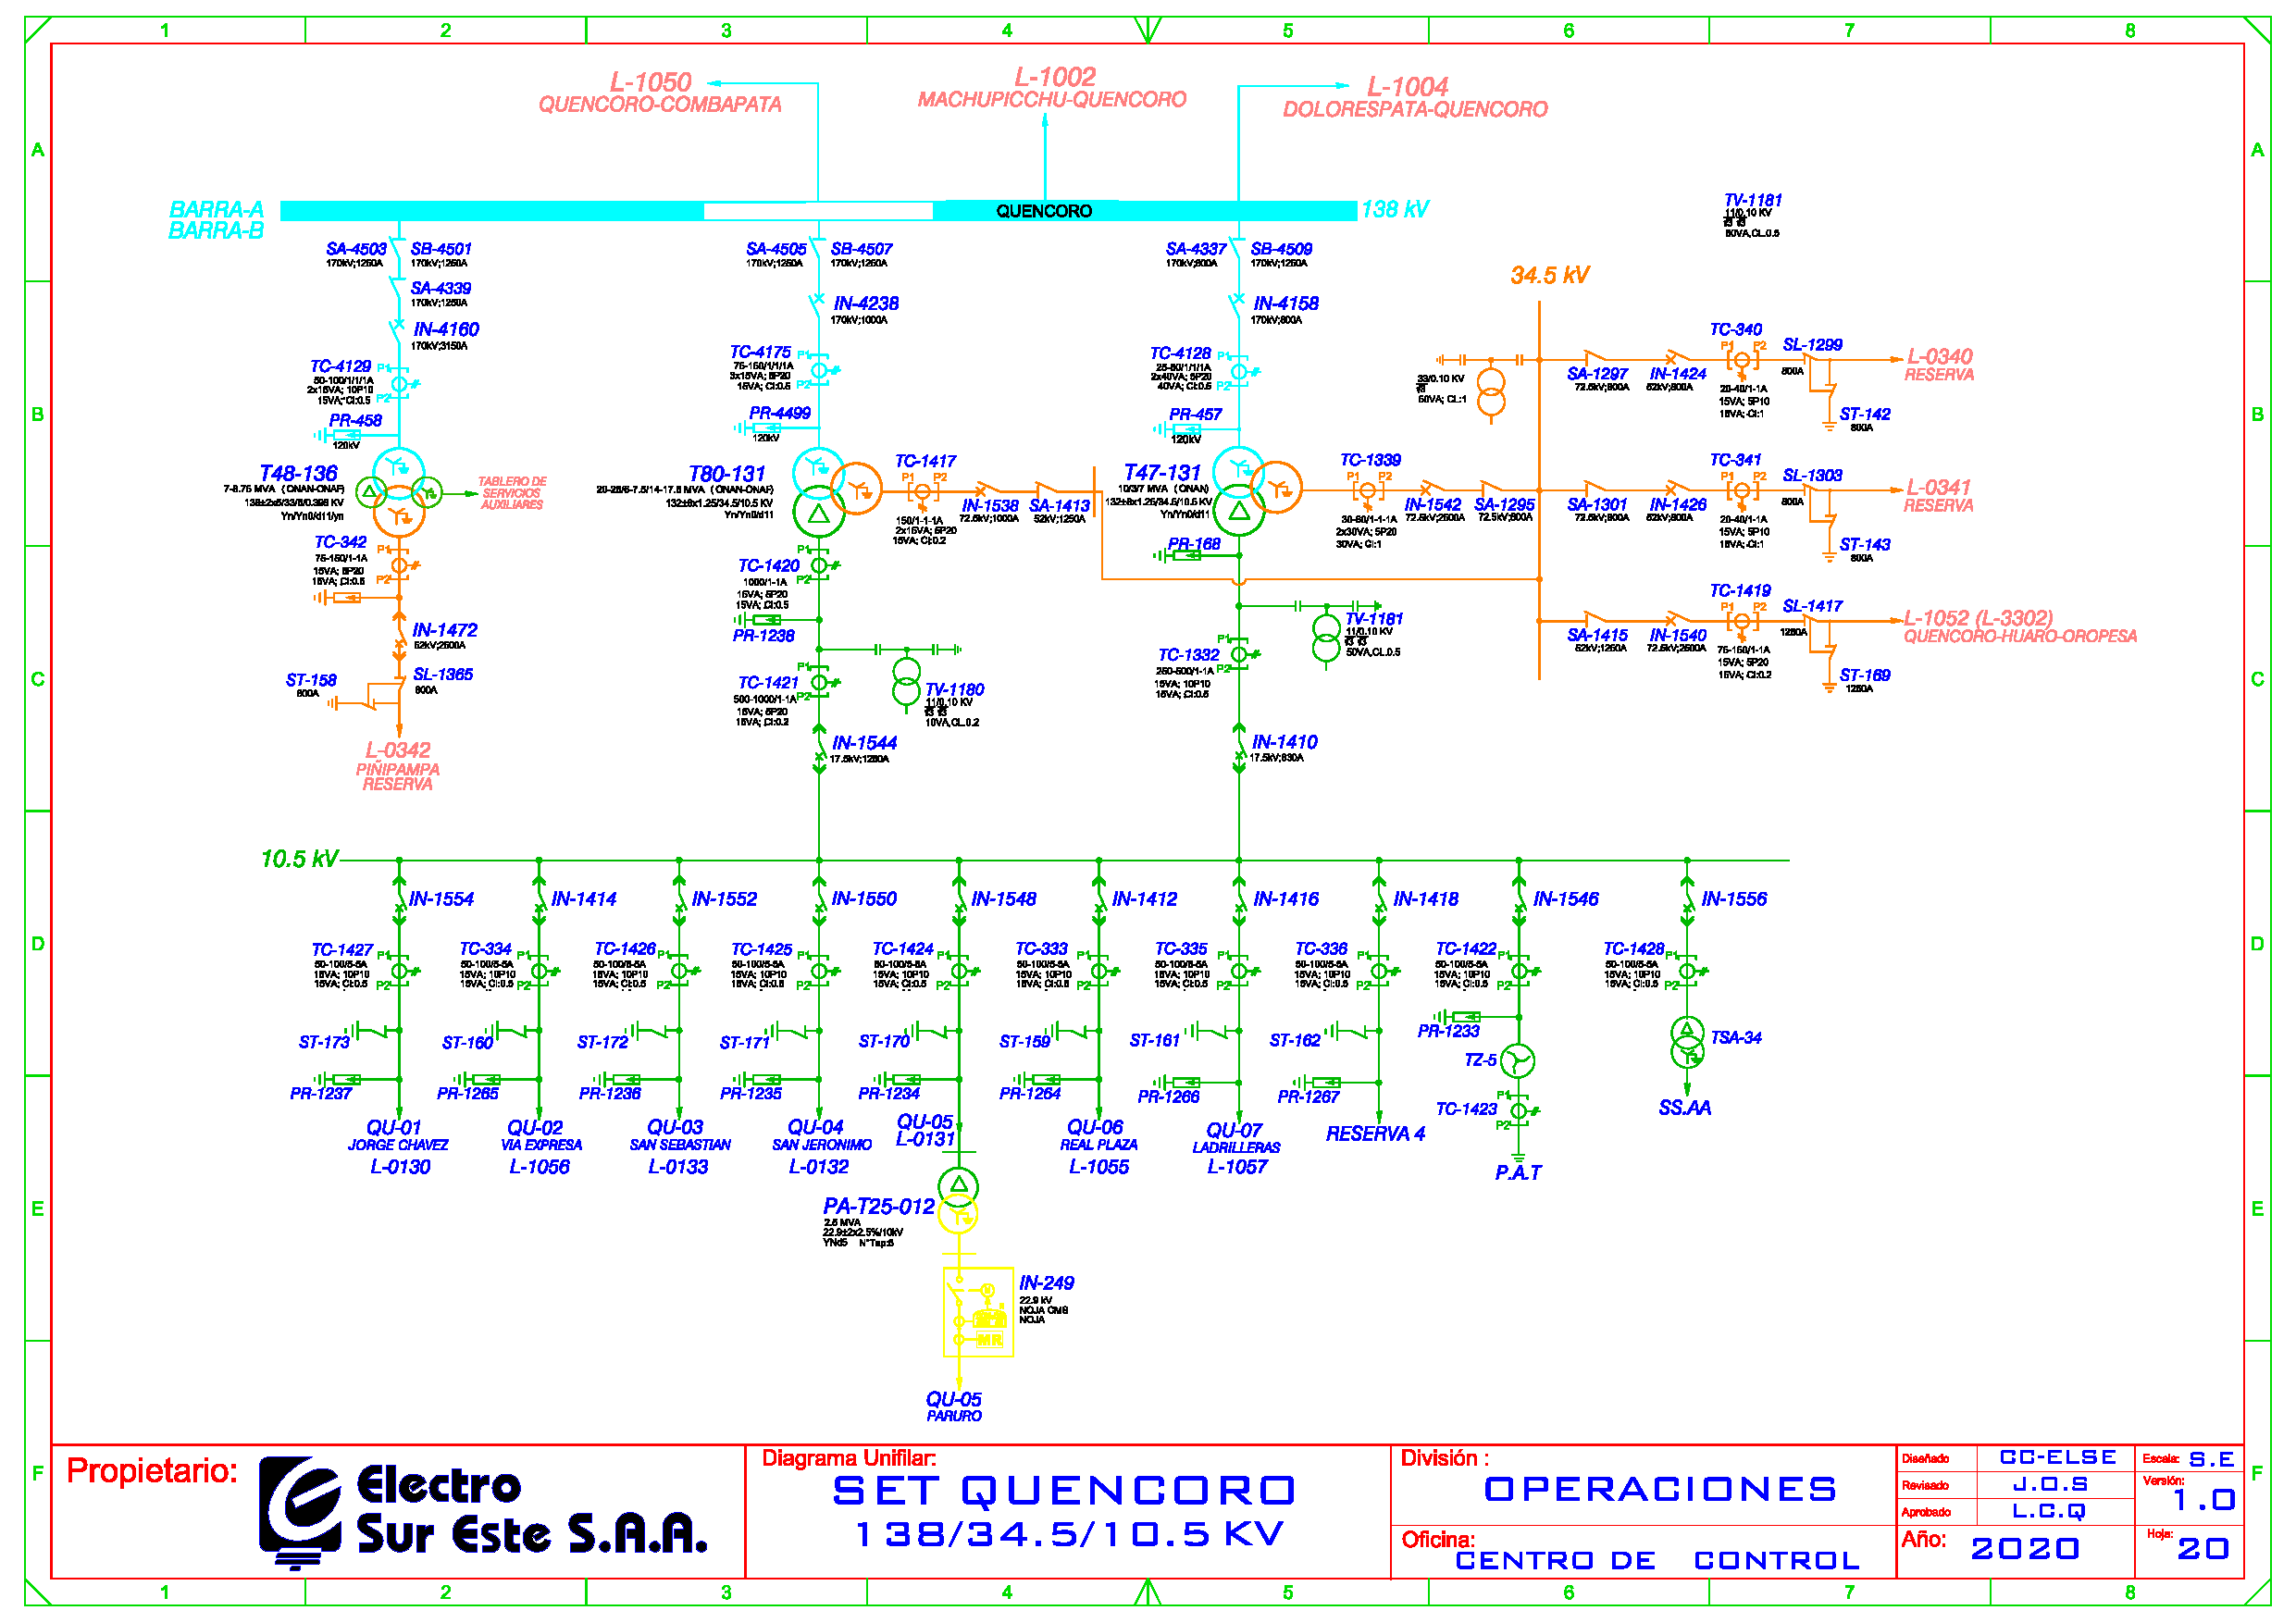
\includegraphics[height=0.9\textheight]{./Figures/SE_QUENCORO_unifilar.pdf}
        \caption{Unifilar diagram of the Quencoro substation}
        \label{fig:unifilar}
    \end{figure}
\end{landscape}

\section{Topology of the SED022 distribution network}
\label{appndx:topology}

\begin{figure}[!t]
    \centering
    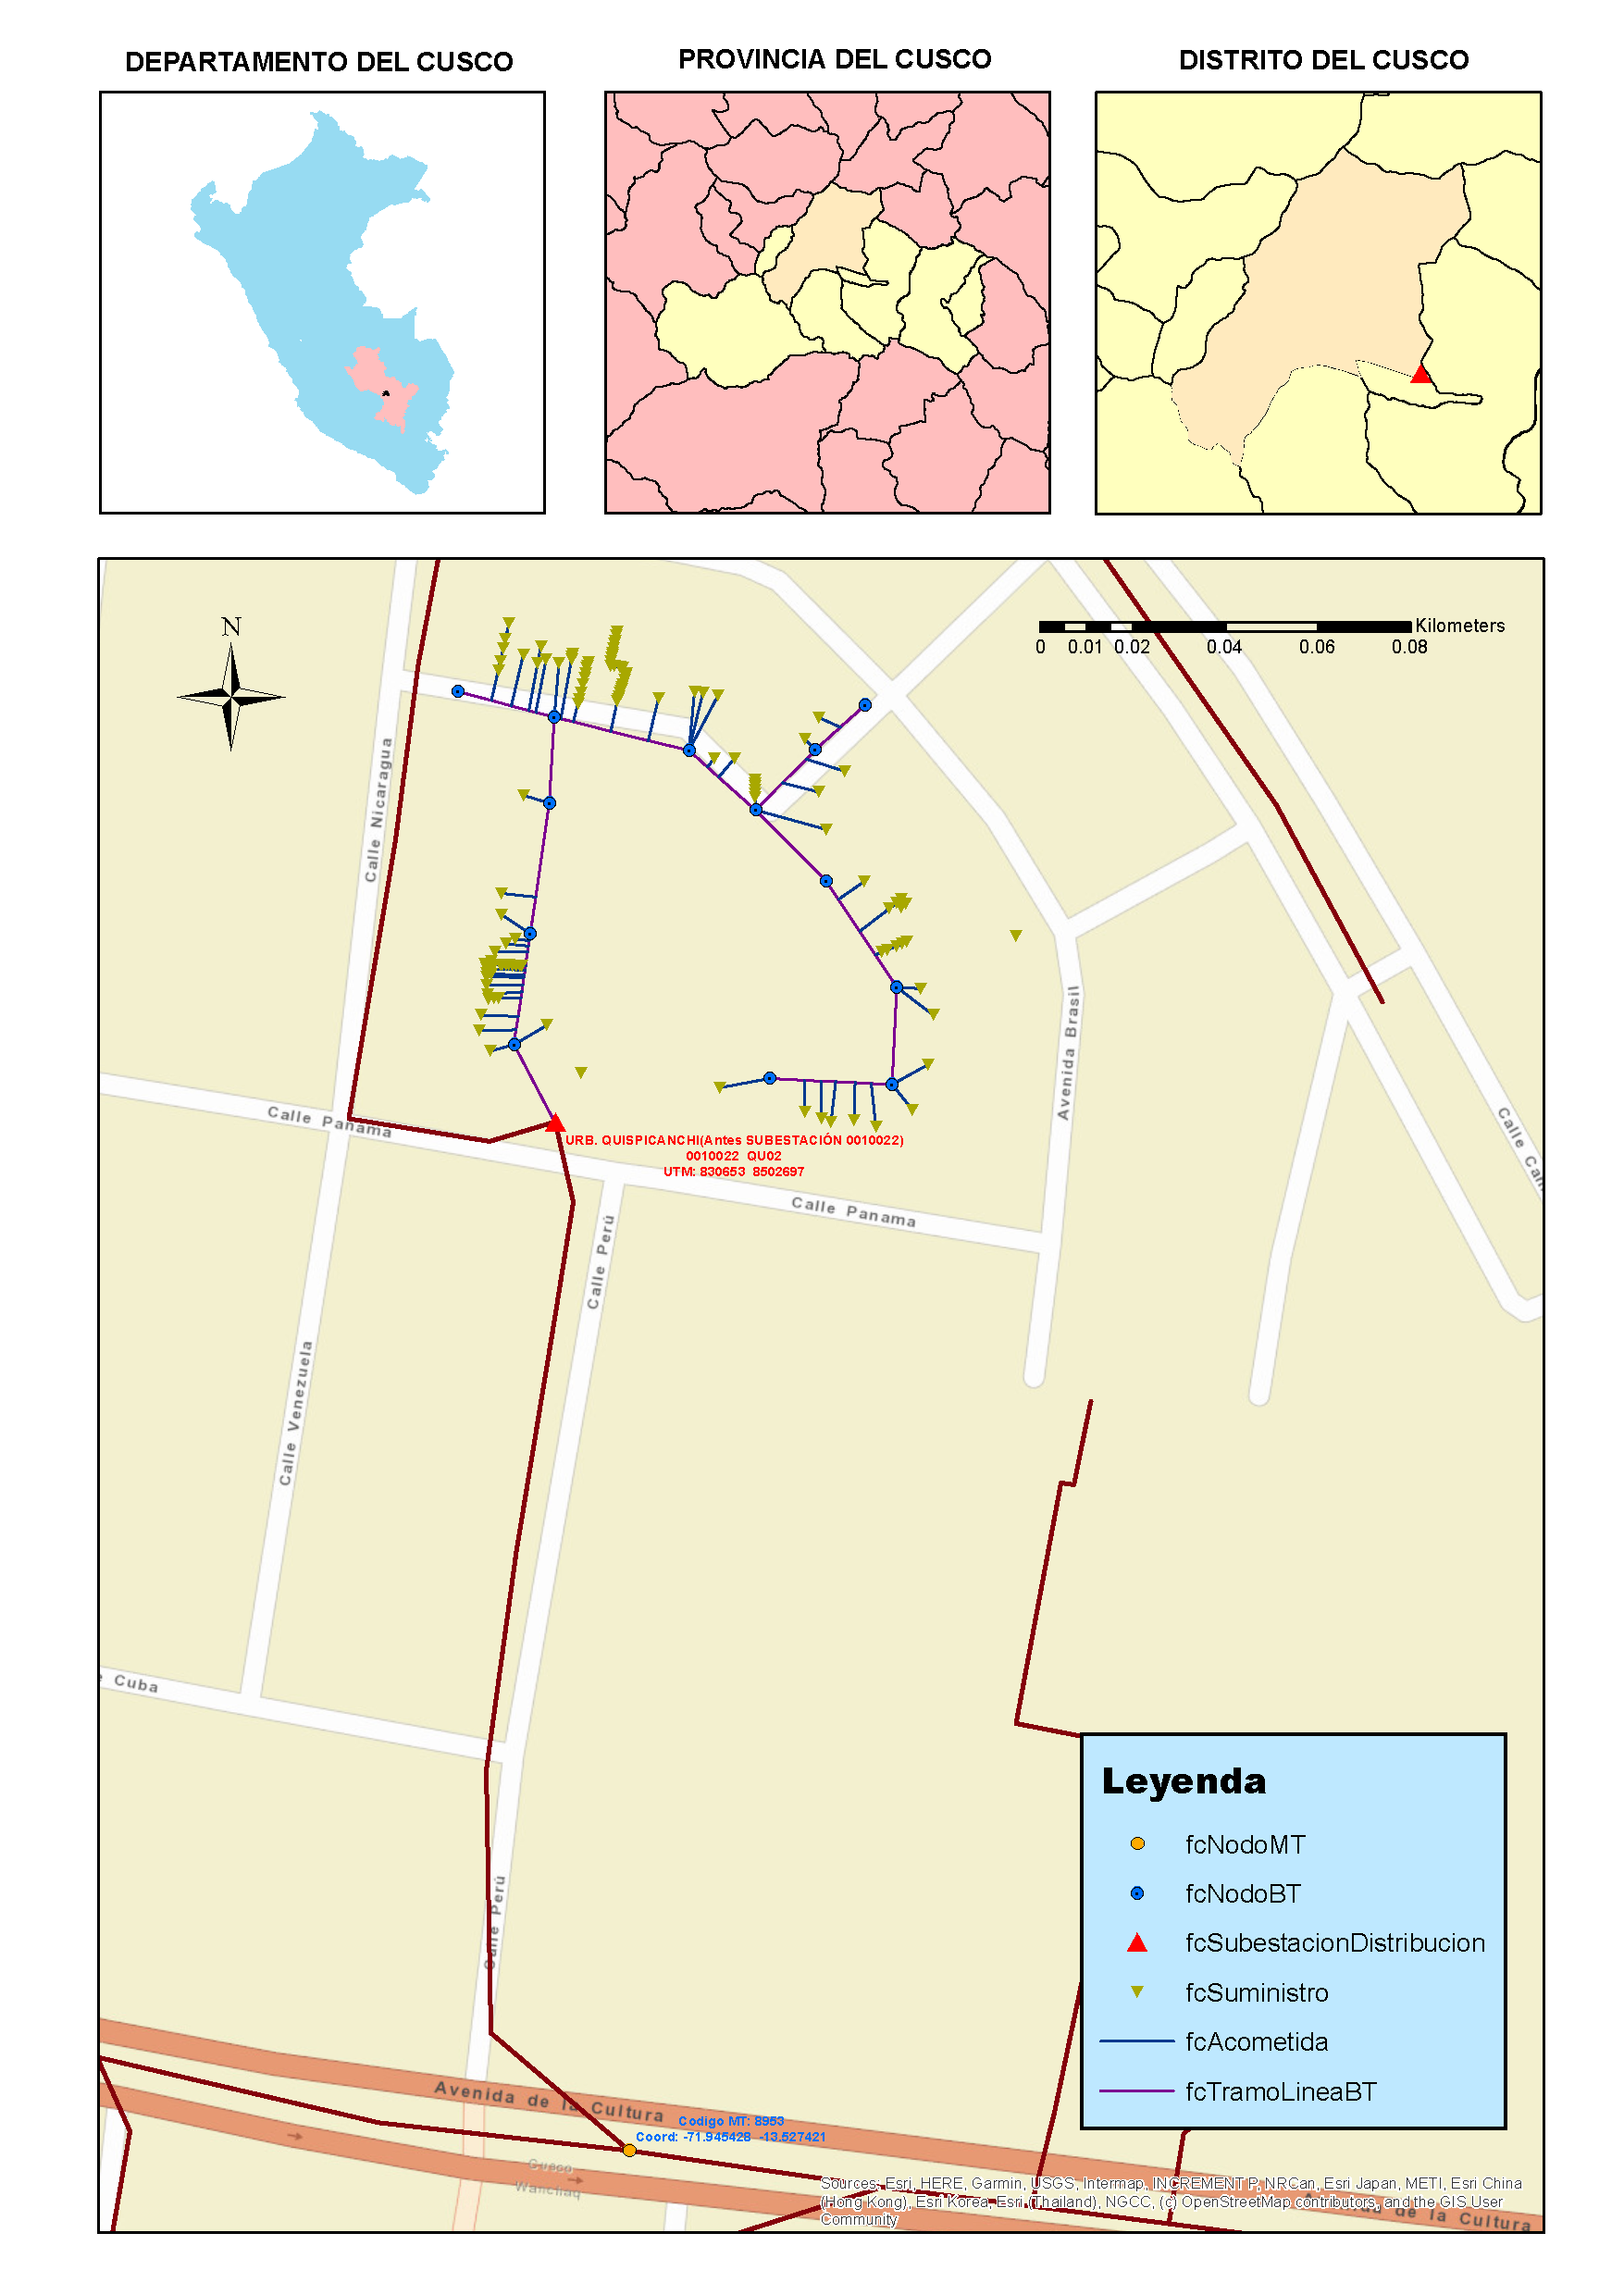
\includegraphics[width=0.8\textwidth]{./Figures/SED_0010022.pdf}
    \caption{Topology of the SED022 distribution network}
    \label{fig:topology}
\end{figure}

\section{Repository with the data and code used in this work}
\label{appndx:repository}

\url{https://github.com/DerianTairoGarcia/Trabalho_final_IT305_H.git}

\bibliographystyle{elsarticle-num}
\bibliography{references.bib}


\end{document}